\subsubsection{Instance Reduction Analysis}
\label{subsubsec:discussion-reduction}

This section interprets the results of the dimensionality reduction techniques, 
discussing their impact on the analysis and visualization.

Figure [INSERT FIGURE REF] shows the results of our analyzis in terms of accuracy, 
training speed and storage reduction capbilities of the instance reduction techniques
 implemented (\textit{i.e.}, GCNN, ENNTH and DROP3)

 ...

This section examines the impact of three reduction techniques—GGCN, ENNTH, and Drop3—on the performance, training time, testing time, and storage requirements of both the KNN and SVM algorithms.

For KNN applied to the Hepatitis dataset, applying no redcution yields a high F1 score of 0.9483, with moderate storage requirements of 139.5 units and a testing time of 0.0747 seconds. 
The GGCN reduction technique slightly lowers the F1 score to 0.9354 but significantly improves testing time to 0.0545 seconds and reduces storage to 103.2 units. 
GGCN achieves this by selectively condensing the dataset, retaining instances that best represent the overall data structure and class boundaries. 
By removing redundant points that do not impact classification accuracy, it effectively reduces storage requirements and enhances processing speed without sacrificing much performance.

The F1 score for ENNTH is the same as applying no reduction, and achieves the fastest training time of 0.00042 seconds, but results in almost no reduction in storage since its approach primarily focuses on removing noisy data points at the boundaries. 
Given the relatively low noise in the Hepatitis dataset, ENNTH performs similarly to applying not reduction in terms of storage efficiency. 
Conversely, Drop3 reduces storage to 110.9 units but leads to a more significant drop in the F1 score to 0.9157. 
This reduction in performance can be attributed to Drop3's aggressive removal of instances based on noise and redundancy filtering, which can inadvertently discard valuable data points and degrade predictive accuracy when the dataset is sparse.

When analyzing the Mushroom dataset with KNN, all techniques achieve a perfect F1 score of 1.0, indicating no loss in predictive accuracy. 
GGCN stands out by significantly reducing storage from 7311.6 units to 3519.8 units while also decreasing testing time from 72.78 seconds to 33.70 seconds. 
This effectiveness arises from GGCN's ability to eliminate redundancy while retaining essential data points, making it particularly advantageous for large datasets. 

ENNTH and Drop3 retain the same storage requirement as the control, both at 7311.6 units, with only slight improvements in training and testing time. 
ENNTH preserves the perfect F1 score by focusing on noise removal, which is less impactful in this dataset due to its inherent cleanliness. 
Similarly, Drop3 achieves a perfect F1 score, as its filtering approach does not affect the well-structured Mushroom dataset.

\begin{figure}
    \centering
    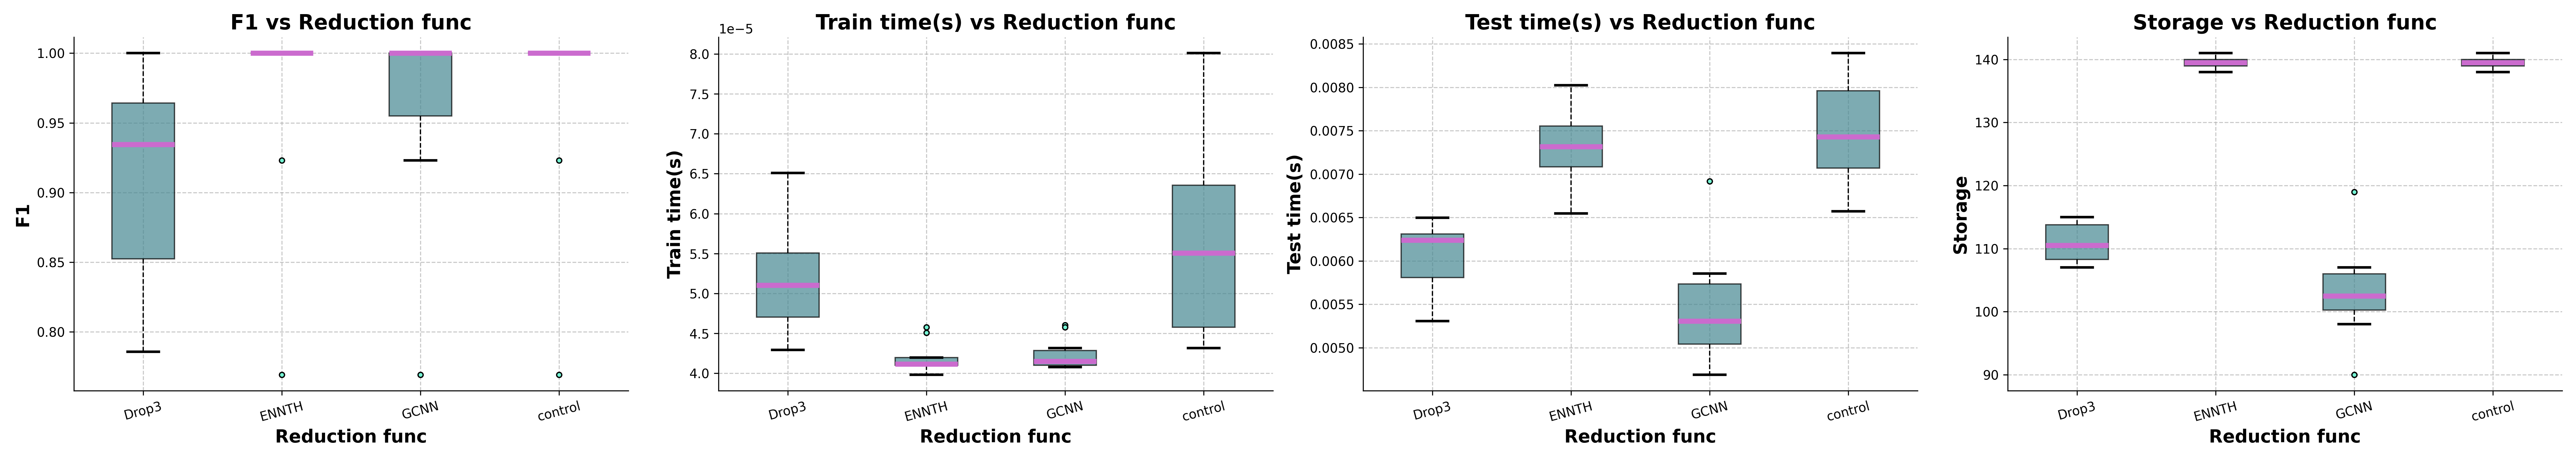
\includegraphics[width=0.45\textwidth]{figures/KNN_reduction_effects_hepatitis.png}
    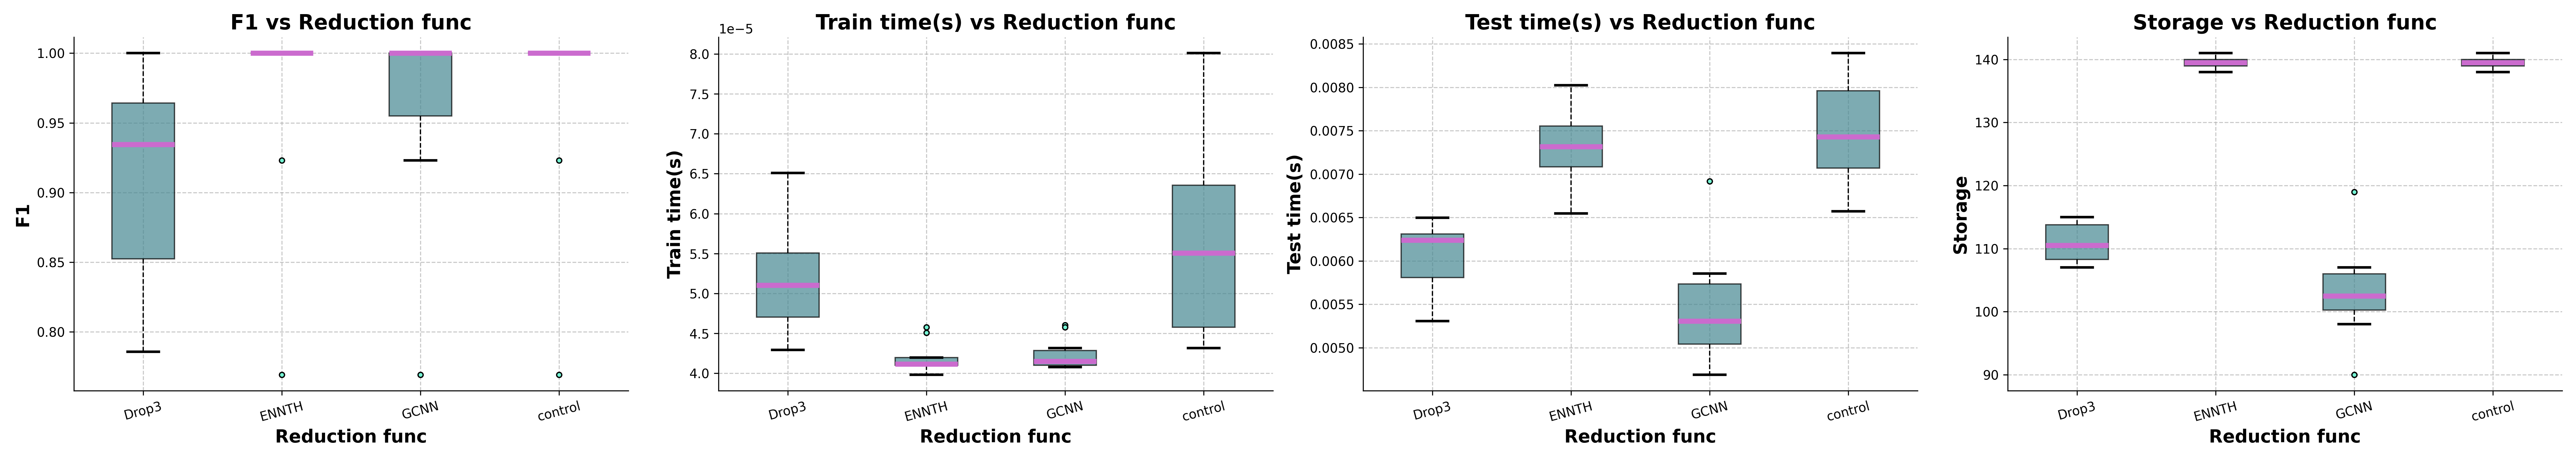
\includegraphics[width=0.45\textwidth]{figures/KNN_reduction_effects_hepatitis.png}
    \caption{Class distributions}
    \label{fig:KNN-reduction-effects}
\end{figure}

In the context of the Hepatitis dataset using SVM, using no reduction method produces a high F1 score of 0.9719, requiring moderate storage of 139.5 units and a testing time of 0.0037 seconds.
The GGCN technique yields a slightly lower F1 score of 0.9597, but it reduces storage to 103.2 units while maintaining a similar testing time of 0.0037 seconds.

ENNTH maintains the original F1 score of 0.9719 and achieves a testing time of 0.0033 seconds, but it results in almost no storage reduction, as its approach primarily focuses on eliminating noisy boundary points. 
The relatively low noise in the Hepatitis dataset means ENNTH performs comparably to the control in terms of storage usage.
On the other hand, Drop3 reduces storage to 110.9 units but results in a substantial drop in F1 score to 0.9291, reflecting its aggressive filtering approach, which can lead to the loss of critical instances and, consequently, a decline in predictive performance.

For SVM applied to the Mushroom dataset, all methods, yield a perfect F1 score of 1.0, ensuring no predictive accuracy is sacrificed. 
GGCN proves especially effective by reducing storage from 7311.6 units to 3519.8 units and decreasing testing time from 0.0421 seconds to 0.0337 seconds.

ENNTH and Drop3 maintain the same storage requirements as the control, both at 7311.6 units, with minor improvements in training and testing time.
ENNTH's focus on noise removal contributes to its sustained perfect F1 score, while Drop3's method similarly does not impact storage significantly in this densely populated dataset.

\begin{figure}
    \centering
    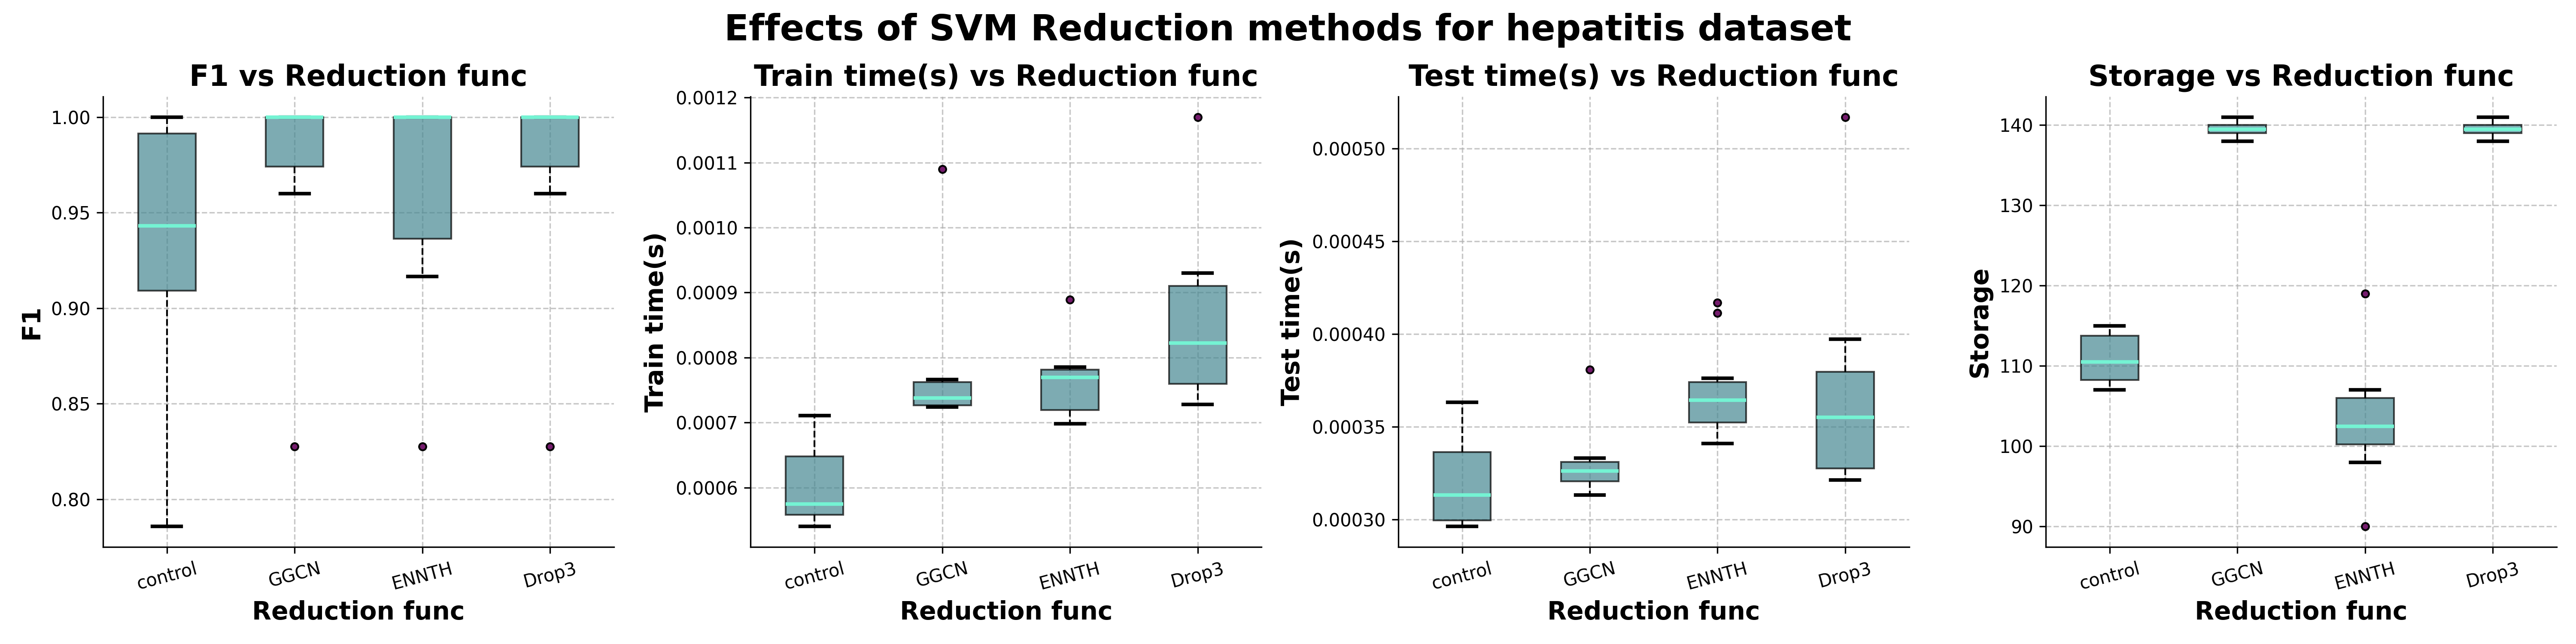
\includegraphics[width=0.45\textwidth]{figures/SVM_reduction_effects_hepatitis.png}
    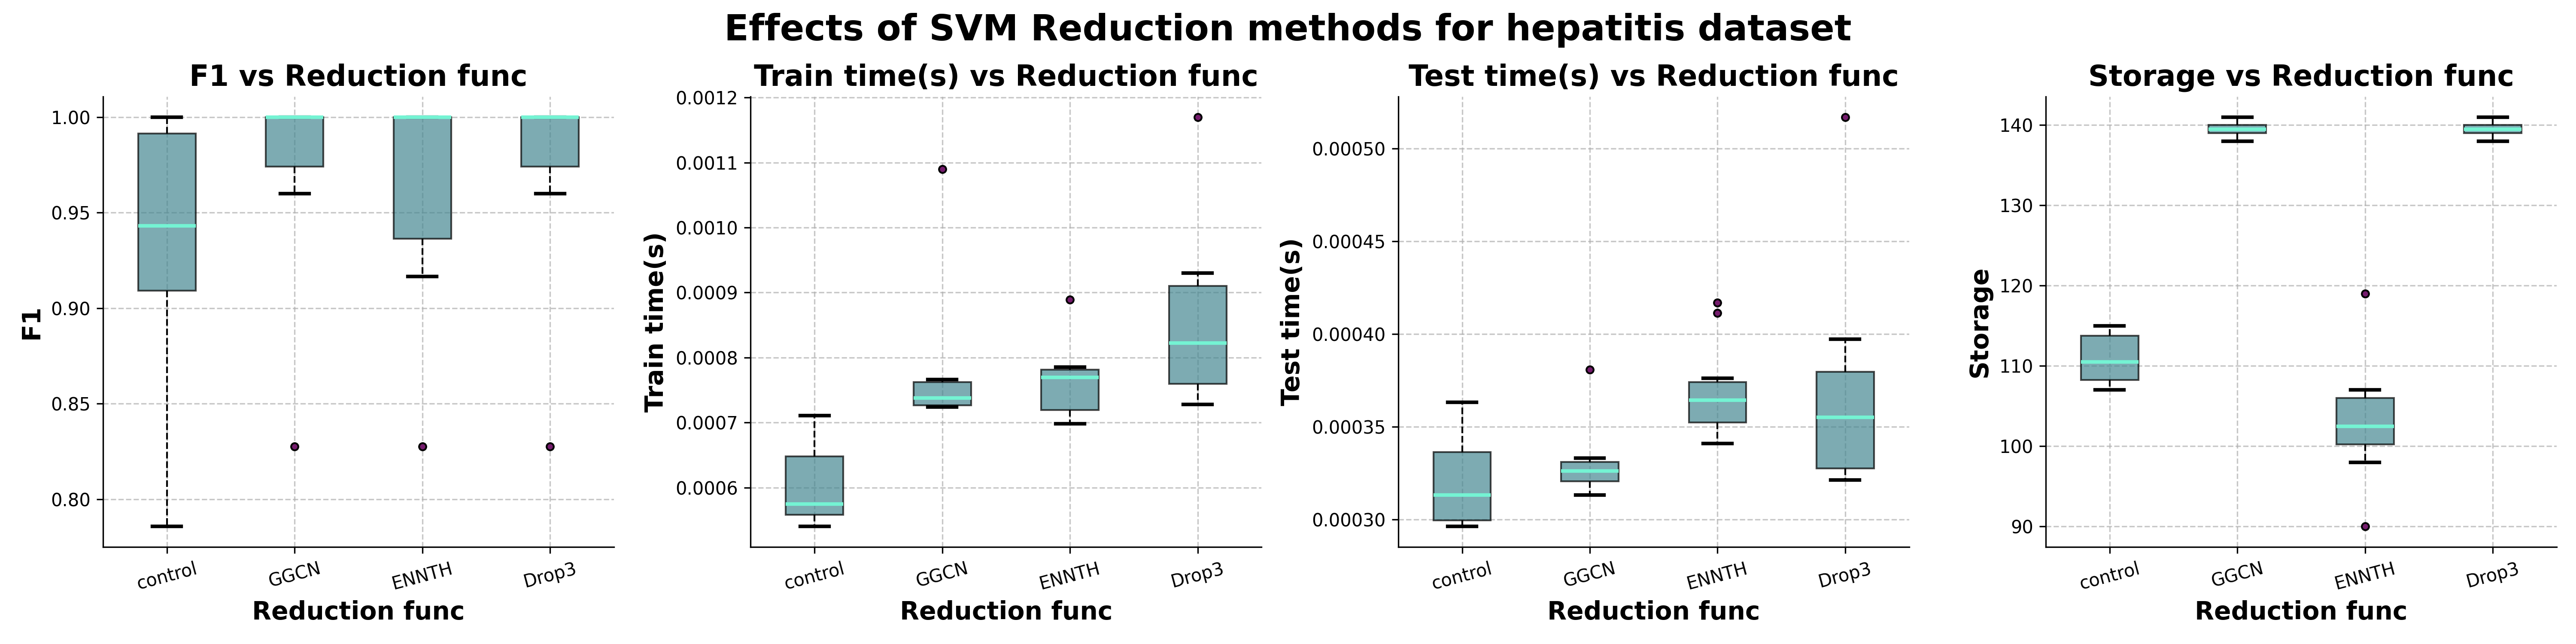
\includegraphics[width=0.45\textwidth]{figures/SVM_reduction_effects_hepatitis.png}
    \caption{Class distributions}
    \label{fig:SVM-reduction-effects}
\end{figure}

Overall, GGCN emerges as the most effective reduction technique across both models, showcasing substantial efficiency gains while preserving predictive accuracy, particularly for larger datasets like Mushroom.


